
\onecolumn

\begin{center}
    {\LARGE \textbf{Supplementary Material for RWKV-X}}\\[2em]
\end{center}

\section{Data and Hyperparameters}
\label{sec:data_Hyperparameters}

\paragraph{Training Data}
RWKV-X training is divided into two phases. 
The first phase, the Alignment Phase, uses the minipile dataset with 1.5 billion tokens. 
The second phase, the Long Context Phase, draws randomly sampled data from the ProLong-64K dataset with a total of 40 billion tokens.

\paragraph{Hyperparameters}
The following hyperparameters were used to train a range of RWKV-X models, from 0.22B to 3.6B parameters, as shown in Table \ref{tab:hyperparameter}.

\begin{table}[h!]
\centering
\resizebox{\textwidth}{!}{
\begin{tabular}{l|cc|cc}
\toprule
\multirow{2}{*}{Hyperparameter} & \multicolumn{2}{c|}{0.22B Model} & \multicolumn{2}{c}{3.6B Model} \\
\cmidrule(lr){2-5}
& Alignment & Long Context & Alignment & Long Context \\
\midrule
Batch size (tokens) & - & 8.192M & 4.096M & 1.024M \\
Context length (tokens) & - & 64,000 & 4,096 & 64,000 \\
Tokens trained (B) & - & 20 & 1.5 & 1 \\
Initial learning rate & - & 1e-5 & 1e-5 & 1e-5 \\
Final learning rate & - & 1e-5 & 1e-5 & 1e-5 \\
Learning rate schedule & - & Constant & Constant & Constant \\
Warmup ratio & - & 0 & 0 & 0 \\
Weight decay & - & 0 & 0 & 0 \\
Optimizer & - & AdamW & AdamW & AdamW \\
DeepSpeed stage & - & 1 & 1 & 1 \\
GPU Configuration & - & 8×H20 & 4×H20 & 8×H200 \\
Total GPU Hours (h) & - & 576 & 6 & 80 \\
\bottomrule
\end{tabular}
}
\caption{Training hyperparameters and compute configurations for RWKV-X models.}
\label{tab:hyperparameter}
\end{table}


\section{Training Efficiency}

Figure~\ref{fig:train_efficiency} illustrates the training efficiency comparison between RWKV-X and RWKV-7 across varying sequence lengths, ranging from 1K to 32K tokens.
As the sequence length increases, both models exhibit approximately linear growth in computation time, consistent with their underlying design. 
Notably, RWKV-X consistently demonstrates lower computation time compared to RWKV-7 at all sequence lengths, highlighting its improved training efficiency. 
The gap in efficiency becomes more pronounced at longer sequence lengths, suggesting that the architectural modifications in RWKV-X more effectively scale with context size. 
These results indicate that RWKV-X offers a more computationally efficient alternative to RWKV-7, particularly for tasks requiring long-context processing.

\begin{figure}[h!]
    \centering
    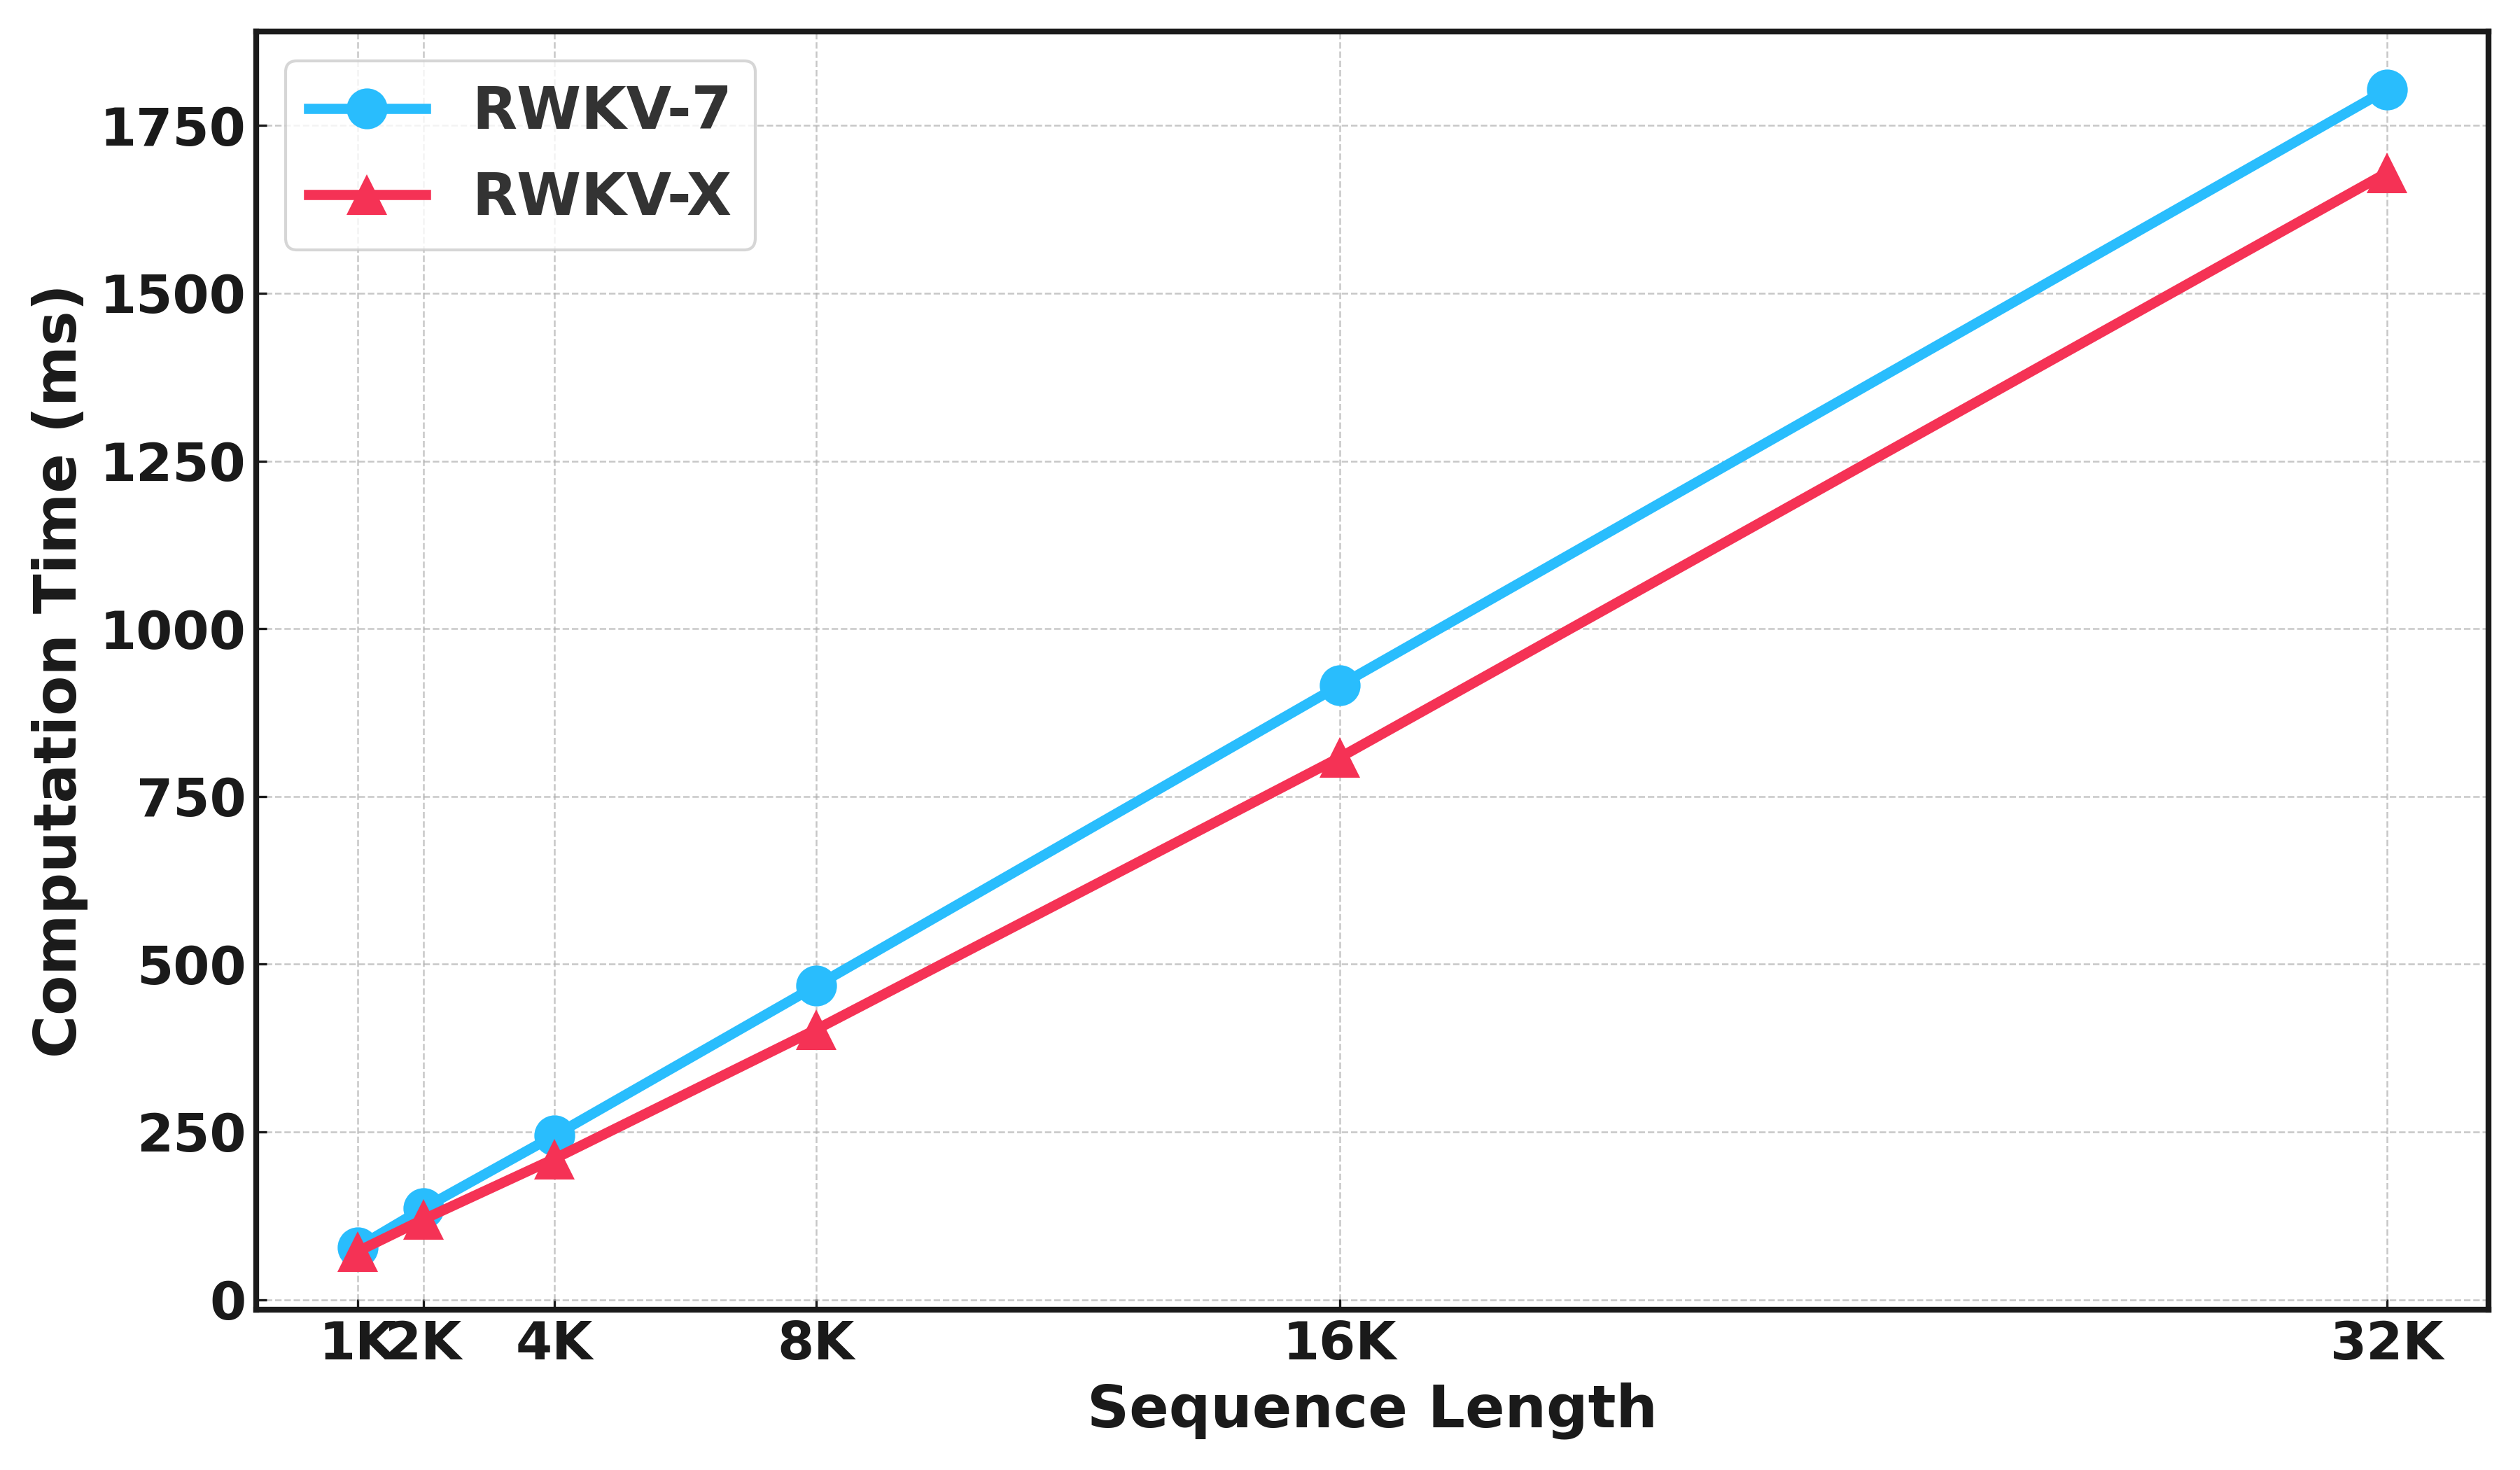
\includegraphics[width=0.7\linewidth]{figures/train_efficiency.png}
    \caption{Training efficiency comparison between RWKV-X and RWKV-7}
    \label{fig:train_efficiency}
\end{figure}

\section{More on Efficiency Analysis}
\subsection{Comparison of Sparse and Full Attention}
Table~\ref{tab:attention-comparison} presents a comparison between sparse and full attention used in RWKV-X across varying context lengths in terms of latency and memory consumption. Sparse attention exhibits slightly higher prefill latency at shorter context lengths, but shows a clear advantage in decoding latency at larger scales (e.g., 121.99 ms vs. 170.79 ms at 256k context length). Memory usage is nearly identical between the two methods for smaller contexts, but sparse attention maintains a slight efficiency lead as the sequence length increases. Notably, sparse attention provides more consistent decoding performance as context length scales, making it more suitable for long-context applications where decoding speed is critical.

\begin{table}[htbp]
\centering
\caption{Comparison of Sparse and Full Attention on Latency and Memory Usage}
\resizebox{\textwidth}{!}{
\begin{tabular}{lcccc}
\toprule
Context Length & Latency (Prefill) & Memory (Prefill) & Latency (Decoding) & Memory (Decoding) \\
               & Sparse / Full     & Sparse / Full     & Sparse / Full       & Sparse / Full      \\
\midrule
4K     & 517.64 / 511.06    & 8.70 / 8.70     & 41.73 / 41.82     & 8.42 / 8.42 \\
8K     & 643.26 / 660.30    & 9.06 / 9.06     & 39.14 / 34.33     & 8.77 / 8.72 \\
16K    & 1408.31 / 1404.56  & 9.66 / 9.66     & 36.04 / 34.31     & 9.45 / 9.32 \\
32K    & 2960.36 / 2955.05  & 10.96 / 10.96   & 37.03 / 34.39     & 10.81 / 10.69 \\
64K    & 6107.07 / 6103.40  & 13.69 / 13.69   & 38.28 / 41.97     & 13.54 / 13.42 \\
128K   & 12913.58 / 12792.79 & 19.20 / 19.20   & 58.59 / 68.14     & 19.06 / 18.93 \\
256K   & 31668.96 / 31776.53 & 30.17 / 30.17   & 121.99 / 170.79   & 30.02 / 29.90 \\
512K   & 95482.76 / 95824.31 & 52.14 / 52.14   & 289.91 / 323.96   & 51.99 / 51.87 \\
\bottomrule
\end{tabular}
}
\label{tab:attention-comparison}
\end{table}


\section{KV Cache Management for Top-\textit{k} Chunk Sparse Attention}
\label{sec:kv_cache}


In Top-$k$ Chunk Sparse Attention, maintaining a manageable KV cache size is crucial for achieving efficient decoding. 
We adopt a compression strategy to ensure that the past KV cache remains constant in size, regardless of the input sequence length.

Figure~\ref{fig:app_kv_cache} illustrates the KV cache management process. 
We begin by splitting the past cache into two parts: the \textit{earlier} cached states $(K_{\text{past}}, V_{\text{past}})$ and the \textit{recent} observation window $(K_{\text{obs}}, V_{\text{obs}})$. The observation window contains the most recent tokens, which are always retained due to their relevance to the current context.

To assess the importance of the earlier cached entries, we calculate a cumulative importance score vector by summing the softmax-normalized attention weights over each key.These scores reflect how much past tokens are attended to by the current observation window. Based on this, we retain the top-$m$ entries with the highest importance, where $m$ is a predefined memory budget. The remaining entries are evicted from the cache.

Following eviction, we update the cache by concatenating the selected top-$m$ keys and values with those from the observation window $(K_{\text{obs}}, V_{\text{obs}})$, producing a compressed cache that preserves essential information while capping memory usage.

Specifically, we dynamically select the most relevant cached entries based on their cumulative attention scores with respect to the observation window queries, and discard less important entries. 
This selective compression significantly reduces memory footprint during long-sequence generation while preserving essential contextual information for accurate predictions.

\begin{figure}[h!]
    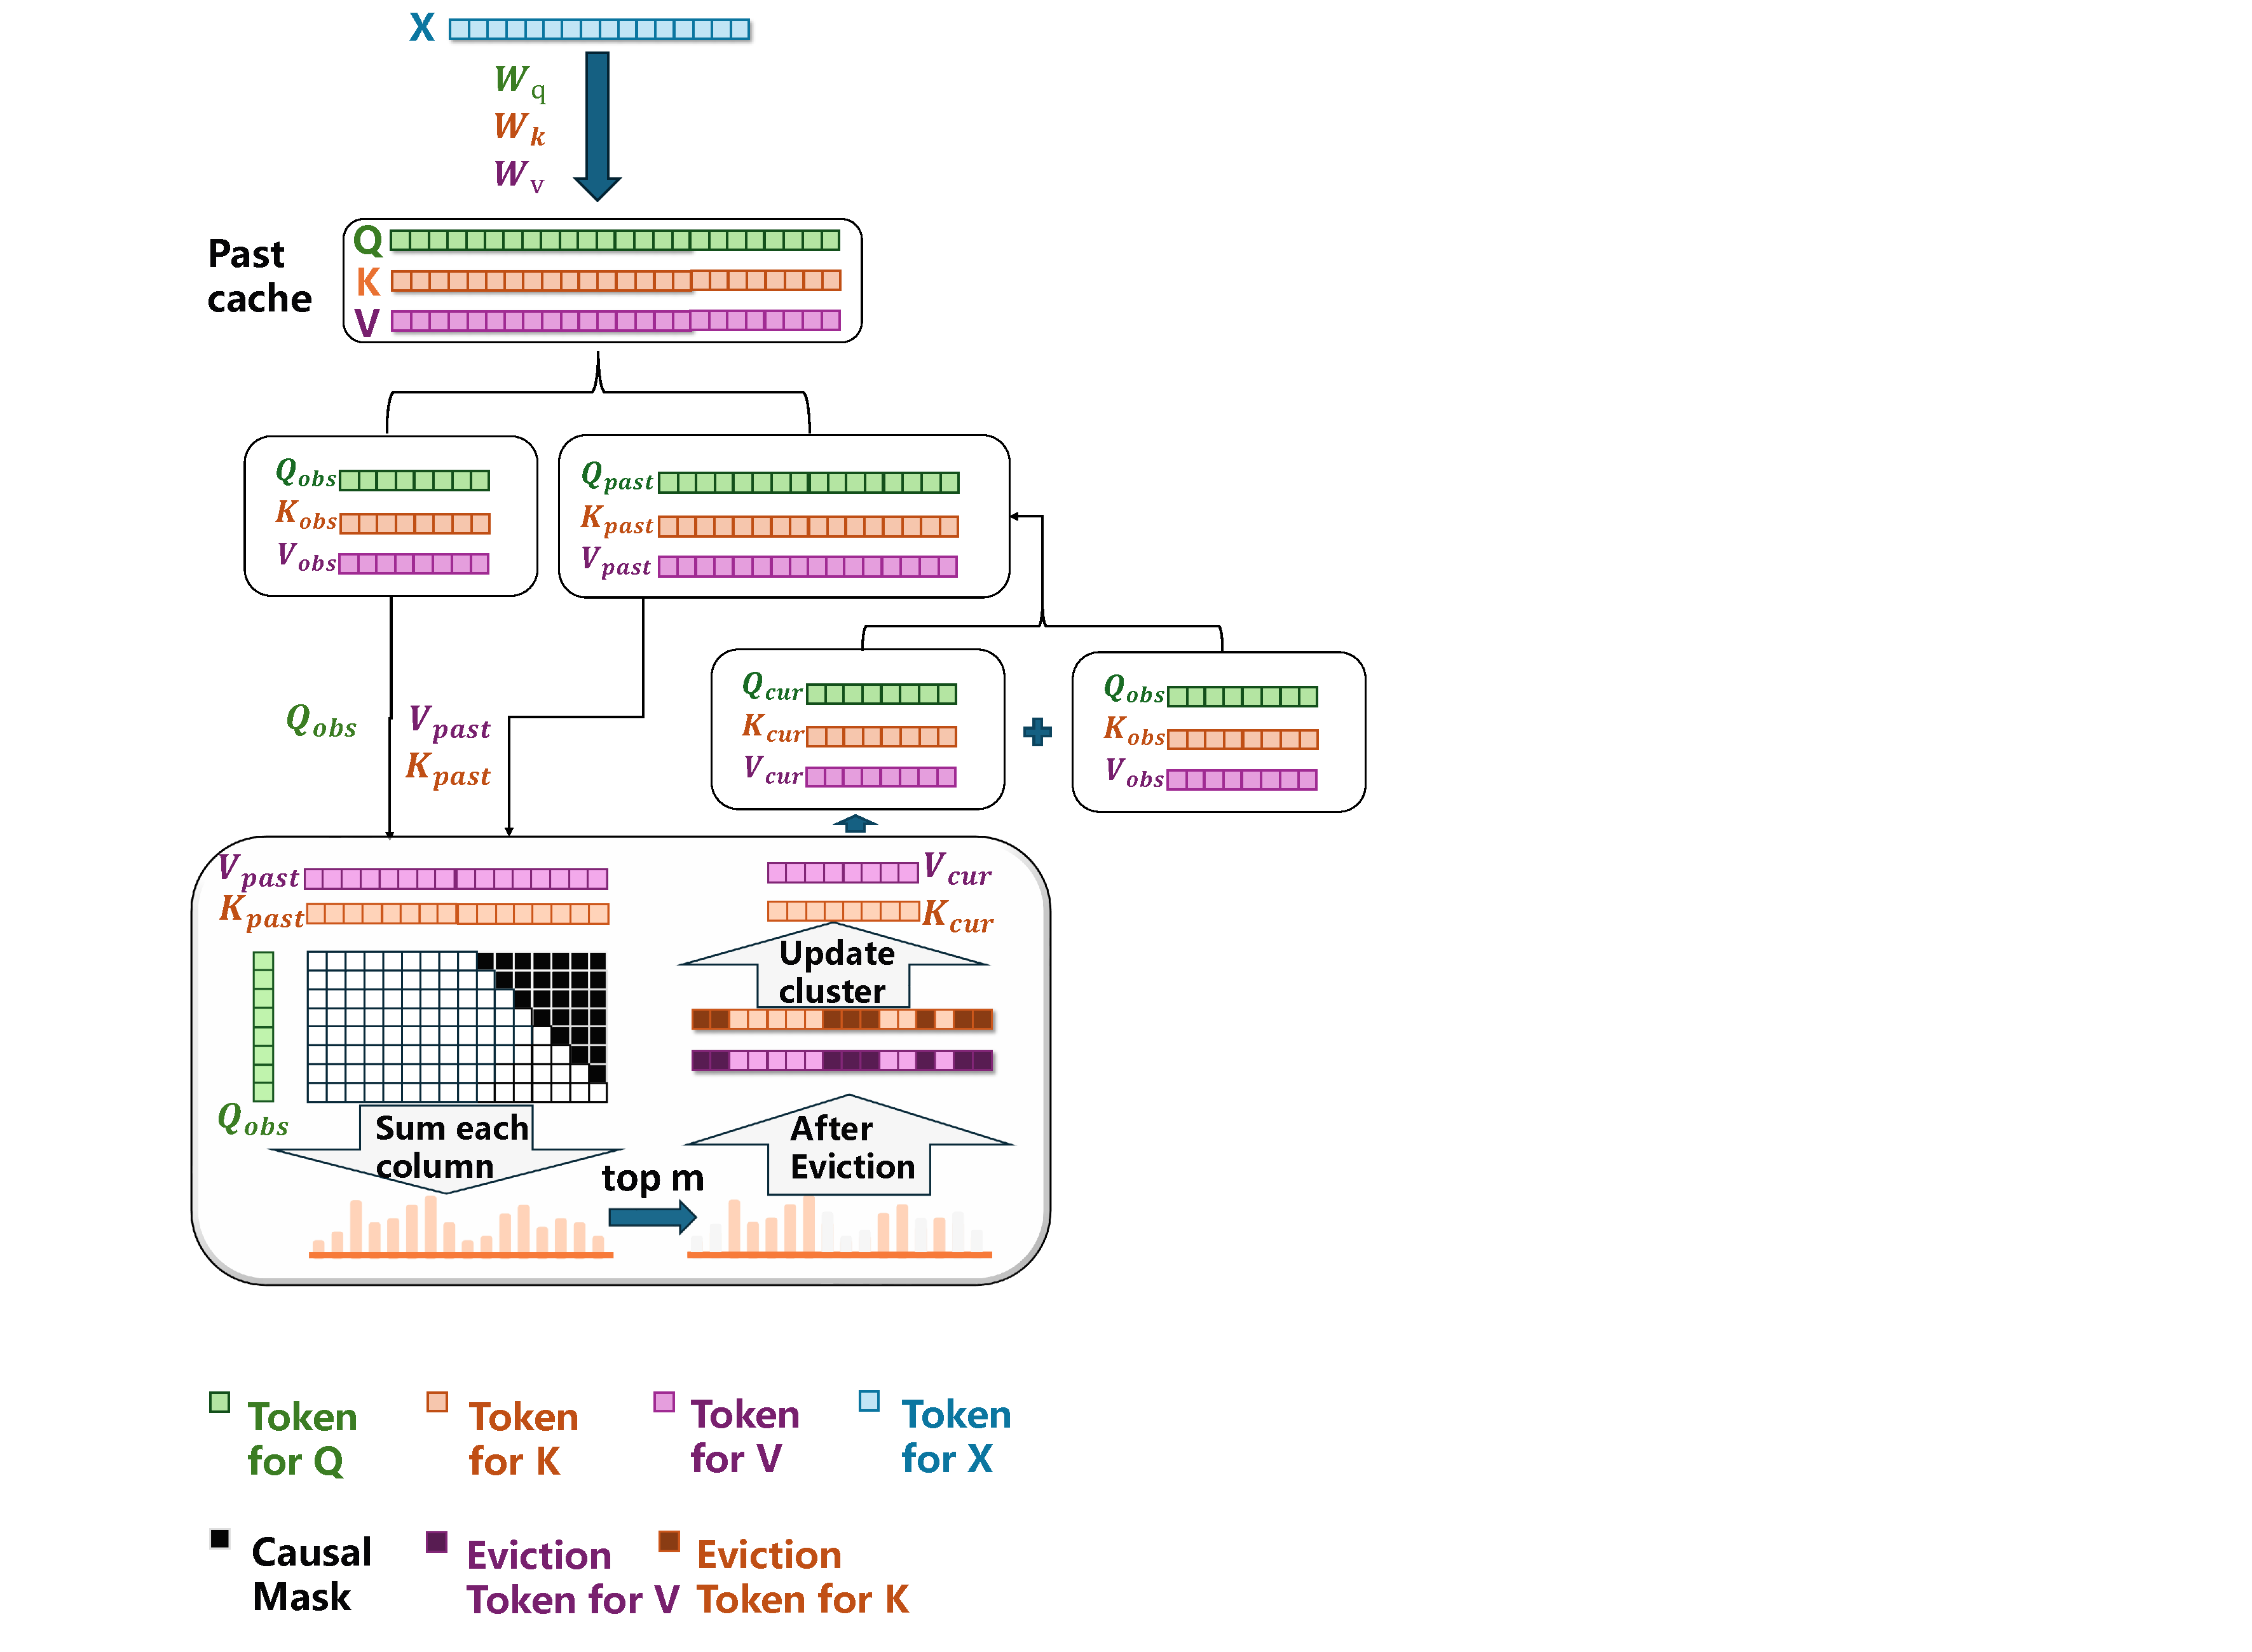
\includegraphics[width=1.5\textwidth]{figures/snapattention.pdf}
    \centering
    \caption{Illustration of KV cache management for Top-$k$ Chunk Sparse Attention.}
    \label{fig:app_kv_cache}
\end{figure}

